
\section{Class System}
\subsection{Outline}

\begin{frame}
  \centering
  {\huge
    Week 1 -- Part 2: How this lecture is organized
  }
\end{frame}

\begin{frame}
  \frametitle{Outline}
  \begin{enumerate}
    \item Class Schedule
    \item Class Materials
    \item How to submit problems
    \item Grading
    \item Office Hours and Teacher Communication
    \item \alert{Special} Distance Learning in 2020
  \end{enumerate}
\end{frame}

\subsection{Class Schedule}
\begin{frame}{What you will do every week}
  \begin{itemize}
    \item (manaba) Get the week PDF and study the lecture;
    \medskip
    \item (manaba) Watch the lecture video;
    \medskip
    \item (OnlineJudge) Read the programming assignments;
    \medskip
    \item Solve the programming assignments;
    \medskip
    \item (OnlineJudge) Test your programs until they are correct;
    \medskip
    \item (manaba) Submit your correct programs;
  \end{itemize}
\end{frame}

\begin{frame}{Class Dates and Deadlines}
  \begin{block}{Class Dates}
    \begin{itemize}
    \item 4/28, 5/12, \alert{5/16}, 5/19, 5/26, 6/2, \alert{6/6}, 6/9, 6/16, 6/23;
    \item No final exam;
    \item Classes will asynchronous (download the video);
    \end{itemize}
  \end{block}
  \begin{block}{Deadlines}
    \begin{itemize}
      \item The deadline for assignments: {\bf 10 days after each week}
      \item The deadline for late assignments: 7/7
      \item Final Grades will be published by 7/13
    \end{itemize}
  \end{block}
  Dates subject to changes.
\end{frame}

\subsection{Class Materials}
\begin{frame}{Lecture Notes and manaba}
  \begin{block}{manaba system}
    \begin{itemize}
      \item Use it to access News, Surveys, and Forums;
      \item Use it to submit assignments;
      \medskip
      \item URL: \url{https://manaba.tsukuba.ac.jp/ct/course_1322213}
      \item Self-registration Code: 6910967 (non-credit students)
    \end{itemize}
  \end{block}
  \begin{block}{github page}
    \begin{itemize}
      \item Has the same material as Manaba (Lecture notes, videos);
      \item Can be accessed by anyone;
      \item CANNOT access news, grades or assigments;
      \medskip
      \item URL: \url{https://caranha.github.io/Programming-Challenges/}
    \end{itemize}
  \end{block}
\end{frame}

\begin{frame}{Websites for programming Assignment}
  \begin{itemize}
    \item {\bf Online Judge}: \url{https://onlinejudge.org}\\
      This website hosts many programming challenges and an Automated Judge.
      In this class, you will submit your programming assignment to this
      site to check its correctness.
    \bigskip

    \item {\bf uMonitor}: \url{https://caranha.github.io/Programming-Challenges/uMonitor/monitor.html}\\
      This website is a javascript that collects information from Online Judge.
      You can use this site to check the assignments for each week, and which
      assigments you have already submitted.
  \end{itemize}
\end{frame}

\begin{frame}{Course Language}
  \begin{block}{Natural Language}
    \begin{itemize}
      \item The materials in this course will be in English;
      \item Announcements and Video Lectures will be in Japanese;
      \item You can use any language you want;
      \item If you are interested in helping translate the materials,
        contact me!
    \end{itemize}
  \end{block}

  \begin{block}{Programming Language}
    \begin{itemize}
      \item The online judge accepts: C, C++, Java, python, PASCAL;
      \item I recommend that you use C++, but you can use other languages;
      \item Code examples in this class will usually be C++;
    \end{itemize}
  \end{block}
\end{frame}

\begin{frame}{Reference Books}
  Textbook:
  \begin{itemize}
    \item {\bf textbook:} Steven Halim, Felix Halim,"Competitive Programming", 3rd edition. \url{https://cpbook.net/}
  \end{itemize}
  \bigskip

  Other references:
  \begin{itemize}
    \item Steven S. Skiena, Miguel A. Revilla,"Programming Challenges", Springer, 2003
    \item 秋葉拓哉、 岩田陽一、 北川宜稔,『プログラミングコンテストチャレンジブック』
    \item 渡部有隆、『オンラインチャレンジではじめるC/C++プログラミング入門、Online Programming Challenge!』 (ISBN978-4-8399-5110-8)
    \item 渡部有隆、『プログラミングコンテスト攻略のためのアルゴリズムとデータ構造』(ISBN978-4-8399-5295-2)
  \end{itemize}
\end{frame}

\subsection{Problem Submission}
\begin{frame}{Submitting Assignments}
  Let's learn how to submit assignments in this lecture. These are the main steps:
  \begin{itemize}
    \item Check the assigment on the monitor page;
    \item Read the assignments on onlinejudge.org and solve them;
    \item Submit the assignment to onlinejudge.org;
    \item Check the results: onlinejudge.org and monitor page;
    \item Submit your code to Manaba;
  \end{itemize}
\end{frame}

\begin{frame}{Submitting Assignments 1}{Check the monitor page}
  \begin{center}
    {\tiny
    \url{https://caranha.github.io/Programming-Challenges/uMonitor/monitor.html}}\\
    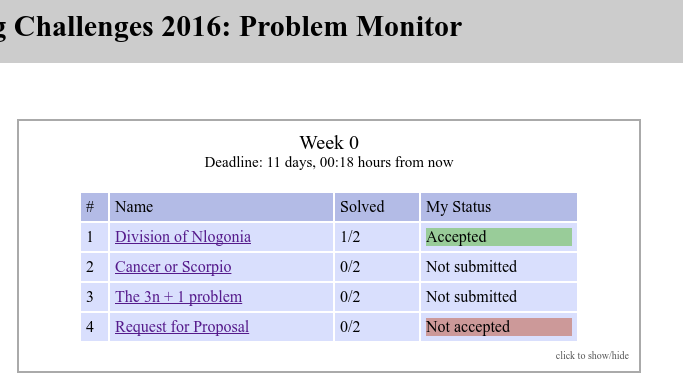
\includegraphics[width=0.5\textwidth]{img/monitorpage}
  \end{center}
  \bigskip

  Check the assignments for each week at the monitor webpage:

  \begin{itemize}
    \item The programming assignments for each week;
    \item The deadlines for each week;
    \item Total submission from the students;
    \item Status of your submissions;
  \end{itemize}
\end{frame}

\begin{frame}{Submitting Assignments 2}{Submitting an assignment to Online Judge}
  Click on a problem name to go to the "Online Judge" page:
  \begin{center}
    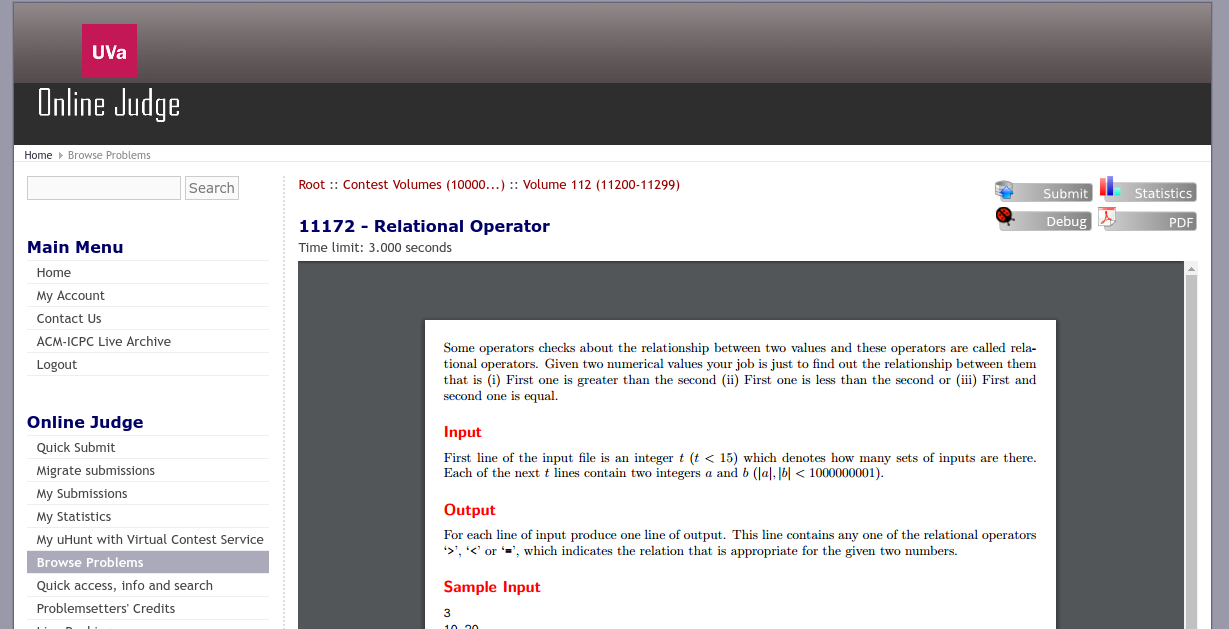
\includegraphics[width=.7\textwidth]{img/relationaloperator}
  \end{center}
  In this page you can get more information about the problem, and submit your code.
  Click on the "submit" button to submit your code.
\end{frame}

\begin{frame}{Submitting Assignments 2}{Submitting an assignment to Online Judge}
  What information can you get from the Online Judge?
  \begin{center}
    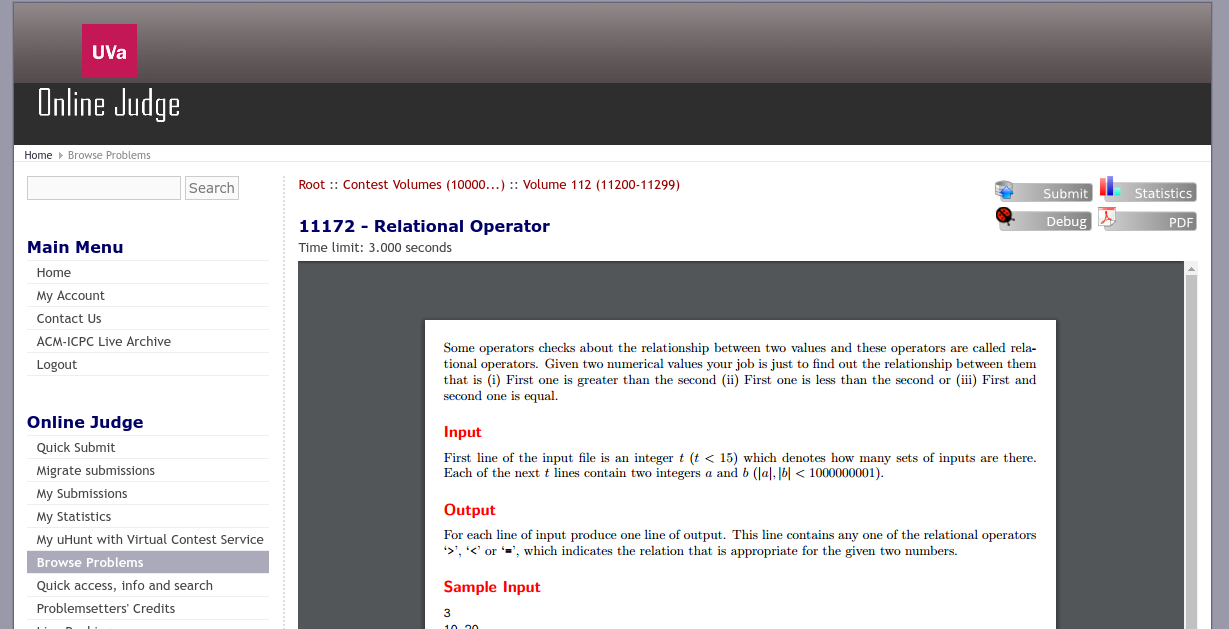
\includegraphics[width=.4\textwidth]{img/relationaloperator}
  \end{center}
  \begin{itemize}
    \item Problem Description -- Read carefully;
    \item Sample Input and Output -- Use this to debug your program;
    \item Time limit -- Make an efficient program!
  \end{itemize}
\end{frame}


\begin{frame}{Submitting Assignments 2}{What is the Online Judge?}

  \begin{block}{What is the Online Judge?}
    \begin{itemize}
      \item Created by the University of Valladolid (Spain);
      \item Now an independent website;
      \item Over 20.000 Programming challenges;
    \end{itemize}
  \end{block}
  \begin{alertblock}{{\bf Important 1: Make an account on Online Judge!}}
    You need an account in Online Judge for this course. When you make your account, {\bf submit your account name on the survey on manaba!}
  \end{alertblock}
  \begin{alertblock}{Important 2: What to do if the judge is offline}
    Sometimes the Online Judge is offline for maintenance. Please be patient.
    If the Online Judge is offline for a long period, there will be a deadline
    extension. This will be announced on manaba.
  \end{alertblock}
\end{frame}

\begin{frame}{Submitting Assignments 3}{Reading the Judge Results}
  \begin{center}
    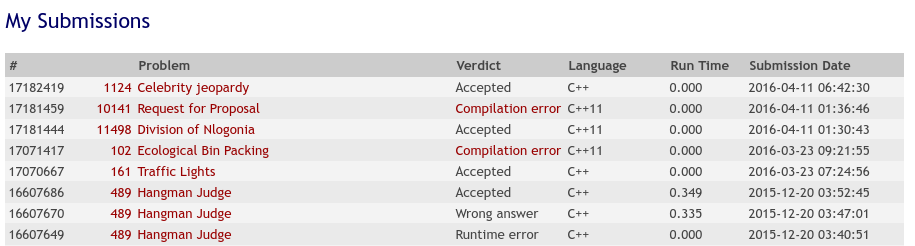
\includegraphics[width=0.8\textwidth]{img/uva_result}
  \end{center}

  \begin{itemize}
    \item After you submit your program, the online judge will evaluate it in 2-5 minutes (or more if it is busy).
    \item You can see the result by clicking on the "my submissions" link;
    \item These are the possible results:
    \begin{itemize}
    \item \structure{Accepted}: Congratulations!
    \item \structure{Presentation Error}: Small mistake. Check the output!
    \item \alert{Wrong Answer}: Your program is incorrect. Time to debug.
    \item \alert{Time Limit Exceeded}: Your program is too slow. Optimize!
    \item \alert{Memory limit exceeded}: Your program uses too much memory.
    \item \alert{Runtime Error}: Your program crashed! (segmentation fault!)
    \end{itemize}
  \end{itemize}
\end{frame}

\begin{frame}{Attention: Java and Python users}
  \begin{block}{Java Users}
  \begin{itemize}
  \item All code must be in the one file;
    \medskip

  \item The \structure{static main} method must be in \structure{Main} class.
    \medskip

  \item Do not use public classes. Even Main must be non public.
    \medskip

  \item Use Buffered I/O for faster input/output.
  \end{itemize}
  \end{block}
  \begin{block}{Python Users}
    Python was added recently to Online Judge. For some of the problems,
    python might be too slow, and maybe you cannot solve in time
    with the same algorithm.
    \medskip

    If you receive too many "Time Limit Exceeded" results, try solving using
    C++;
  \end{block}
\end{frame}

\begin{frame}{Submitting Assignments 3}{Reading the Monitor Results}
  \begin{center}
    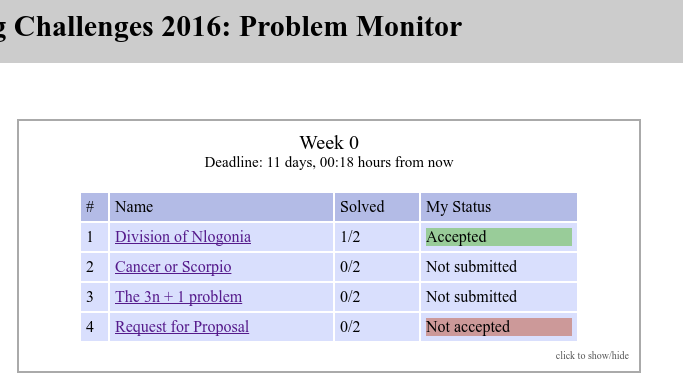
\includegraphics[width=.5\textwidth]{img/monitorpage}
  \end{center}
  \bigskip
  \begin{itemize}
    \item You can check the overall status of your submissions on the
    problem monitor;
    \medskip
    \item This information also include the deadlines for each week, and
    if your submissions are late or not;
    \medskip
    \item This information will only be available after your complete the
    {\bf manaba survey};
  \end{itemize}
\end{frame}

\begin{frame}{Submitting Assignments 4}{Submitting the code to Manaba}
  \begin{itemize}
    \item You must submit your assignment to manaba after you check your code
    is correct;
    \item Put all your program files in a single zip file;
    \item Avoid using non-ascii characters for the filenames;
    \item \alert{Attention:} Do not forget to submit to manaba!
  \end{itemize}
  \bigskip

  \begin{block}{s2020999\_tsukubataro\_w01.zip}
    \begin{itemize}
      \item program1.cpp
      \item program2.cpp
      \item program3.java
      \item program5.cpp
    \end{itemize}
  \end{block}
\end{frame}

\subsection{Grading}
\begin{frame}{Grading}
  Your grades are calculated based on the number of programs you submit
  \bigskip

  Grade Algorithm: {\bf Base Grade} \alert{-Late Penalty} \structure{+ Rank Bonus}

\end{frame}

\begin{frame}{Grading}{Base Grade}
  Every week, there are 8 programming assignments. You don't need to solve
  every one (but please try!). Your base grade is based on how many problems
  you solved.

  \begin{itemize}
    \item {\bf Base Grade}:
    \begin{itemize}
      \item "C": Minimum 2 problems per week;
      \item "B": Minimum 3 problems per week;
      \item "A": Minimum 4 problems per week;
    \end{itemize}
  \end{itemize}

  {\bf Warning 1:} Only "Accepted" problems count. Not "Wrong Answer"
  {\bf Warning 2:} The grade is based on minimum problems. Not average.
\end{frame}

\begin{frame}{Grading}{Late Penalty}
  You can still submit your assignment after the weekly deadline.
  However, if you submit too many assignments late, you will receive a penalty.
  \bigskip

  The penalty reduces your grade by one level. A to B, B to C. The penalty
  {\bf will not} reduce your grade below C.
  \bf

  You will receive a penalty if more than 25\% of your assignments were
  submitted late.
\end{frame}

\begin{frame}{Grading}{Rank Bonus}
  For each base grade (C, B, A), 10\% of the students with the most
  {\bf total problems} will receive a bonus.
  \bigskip

  The bonus will raise your base grade. C to B, B to A, A to A+.
  \bigskip

  In very special cases, the professor may give a bonus for a student
  that contributes greatly to the class.
\end{frame}

\begin{frame}{Grading}{Plagiarism}
  The assignments are \alert{individual}. You must write your
  programs by yourself.

  \begin{exampleblock}{You can do this}
    \begin{itemize}
    \item Ask for ideas to your friends;
    \item Ask for ideas in the MANABA forum;
    \item Ask for help with a bug;
    \end{itemize}
  \end{exampleblock}

  \begin{alertblock}{You can NOT do this}
    \begin{itemize}
    \item Copy a solution from the internet;
    \item Copy a solution from your friends;
    \item Give your code to a friend;
    \end{itemize}
  \end{alertblock}

  Students who do plagiarism will fail the course, and possibly
  suffer penalties from the university.
\end{frame}

\subsection{Teacher Communication}
\begin{frame}{Teacher Communication}
  \begin{itemize}
    \item The teacher will use the manaba "News" systems to send important news. Make sure to check if you get a message from manaba;
    \medskip
    \item New class materials will be posted on the github page, and on manaba before the lecture time;
    \medskip
    \item This semester we do not have "real time" lectures, but the professor will reserve the lecture time (Tue 3,4) for "office hours";
    \medskip
    \item Use the manaba "Forums" systems to ask questions about the assignments;
    \medskip
    \item Send an e-mail to the professor with any questions about the course that are not about assignments;
    \medskip
    \item You can send e-mail and forum message in English or Japanese;
  \end{itemize}
\end{frame}

%Special 2020
\begin{frame}{Programming Environment}
  In this lecture, you will need to write and compile programs to complete
  the assignments and get your grade;
  \bigskip

  If you do not have a programming environment (do not have a computer at home),
  and you are a student from the College of Information Science (COINS), the
  college will help you. Please contact the teacher by e-mail;
  \bigskip

  If you are a student from another college, please contact the professor.
  I cannot promise that I can help you, but I will do my best.
\end{frame}

\begin{frame}{Important Reminder}
  For this class, you need an account on the Online Judge website.
  \bigskip

  Please make an account on that website, and submit your username
  on the manaba survey.
  \bigskip

  If you don't complete the survey with your username, you will
  not be graded!
\end{frame}
